\documentclass{report}
\usepackage{cours}

\usepackage{biblatex}
\addbibresource{biblio.bib}

\title{{\small Projet d'Initiation à la Recherche}\\Étude numérique de cas d'instabilités par l'utilisation de métamodèles\\Numerical study of instability cases using metamodels}
\author{Edgar Pierre BURKHART\and\textit{Encadrante:} Amélie FAU}
\date{2019 --- 2020}

\begin{document}

\maketitle

\chapter*{Abstract}

\tableofcontents

\chapter{Determination of instabilities of slender elements}
\section{Introduction}
In this chapter, the goal is to establish instability zones regarding the buckling of columns as welle as flexural-torsionnal buckling of slender elements.
This study will be mainly focused on steel beams and reinforced concrete columns.

\section{Buckling of columns}
Buckling of columns can appear when a slender element is subjected to a compression load.
In this study, only axial centered compressive loads will be considered (Fig.~\ref{fig:flamb}).

\begin{figure}
    \centering
    \begin{tikzpicture}
        \draw (0,0) -- (0,4);
        \draw (-.5,0) -- (.5,0);
        \foreach \i in {-.5,-.4,...,.6} {
            \draw (\i,0) -- ++ (-120:.2);
        }
        \draw[->] (0,5.5) -- (0,4.5) node[above right]{$P$};
    \end{tikzpicture}
    \caption{Axial centered compressive load.}\label{fig:flamb}
\end{figure}

\subsection{Charge d'Euler}
Par un rapide calcul de l'effort minimal avant instabilité d'une poutre comprimée, on obtient \cite{coursfla}:
\begin{dmath}
    P_{cr}=\frac{\pi^2}{k^2L^2}EI
\end{dmath}

Cette charge critique est appelée charge critique d'Euler. Les paramètres dont elle dépend sont:
\begin{itemize}
    \item $l$: longueur de l'élément comprimé,
    \item $E$: module d'Young du matériau utilisé,
    \item $I$: moment d'inertie quadratique de la section,
    \item $k$: paramètre dépendant des liaisons aux extrémités de l'élément étudié.
\end{itemize}

Cette formulation est valable uniquement dans le cas de poutres dont la rigidité de flexion $EI$ ne varie pas selon la portion de la poutre considérée.

Un instabilité apparaît si la charge appliquée est supérieure à la charge critique d'Euler.

Les valeurs de $k$ sont connues pour des appuis classiques. Dans le cas d'un poteau bi-encastré, $k=\num{.5}$ par exemple. Pour un poteau dont les deux extrémités sont libres en rotation, $k=\num{1}$ \cite{coursfla}.

\subsection{Calculs normatifs de l'Eurocode 3}
L'Eurocode 3 \cite{EC3} présente une méthode permettant de déterminer l'effort maximal admissible en tête d'un poteau métallique. Dans ce cas, l'objectif n'est plus de déterminer la présence d'instabilités, mais plutôt le risque de rupture.

Les différents paramètres du modèle sont:
\begin{itemize}
    \item les dimensions du profilé,
    \item les liaisons aux extrémités,
    \item le matériau utilisé (module de Young, résistance).
\end{itemize}

\subsubsection{Résultats}
Voir Figures~\ref{fig:res1}~et~\ref{fig:res2}.

\begin{figure}[!ht]
    \centering
    \includesvg[width=.8\linewidth]{fig/EC3Slen}
    \caption{Eurocode 3, $x=S$, $y=L$.}\label{fig:res1}
\end{figure}

\begin{figure}[!ht]
    \centering
    \includesvg[width=.8\linewidth]{fig/EC3NEdfy}
    \caption{Eurocode 3, $x=N_{Ed}$, $y=f_y$.}\label{fig:res2}
\end{figure}

\subsection{Méthode de Faessel}

La méthode de Faessel est utilisée pour déterminer la résistance d'un poteau en béton armé vis-à-vis du flambement. Cette méthode se base sur l'existence d'un défaut initial sur l'élément. On calcule en fonction de l'excentricité le moment appliqué ainsi que le moment résistant puis on cherche un point d'intersection qui, s'il existe, détermine le point de fonctionnement du système ainsi définit. Si aucun point d'intersection n'existe, la résistance n'est pas assurée.

This method is a general method used to establish the resistance of a reinforced concrete column under buckling loads.
It is a non-linear study  taking into account the geometrical non-linearity as well as the non-linearity of the behavior of the materials.

\subsubsection{Steel reinforcements behavior}
To model the behavior of steel, a curve with a plateau will be considered.

\subsubsection{Concrete behavior}
The behavior of the concrete parts will be modelled using a simplified Sargin diagram.
The effects of stretched concrete will be neglected in this approach.

\subsubsection{Implementation}
The Faessel method will be implemented in Python using the \texttt{NumPy} module in order to have adapted data storage types.
The calculation points will be determined using the Latin-Hypercube Sampling method.

\subsubsection{First results}
Compared to the other methods, this one has a much slower execution time. The fact that non-linear are taken into account make this method much more resource intensive than the other ones.

The first results were obtained with 100 points, with an execution time of over 100 seconds. The resulting diagram is show in Figure~\ref{fig:faessel2}.

\begin{figure}[t]
  \centering
  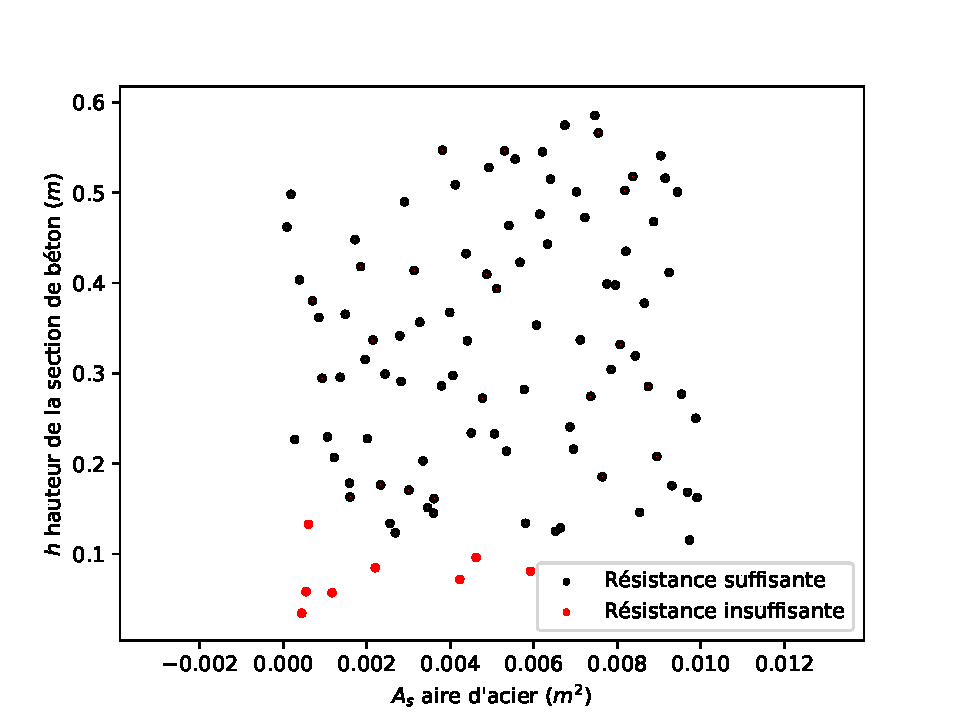
\includegraphics[width=.6\linewidth]{fig/faessel2}
  \caption{First results obtained with the Faessel method (N=100).}\label{fig:faessel2}
\end{figure}

In order to get better results, another calculation was done with \num{1000} points, giving more accurate results at the cost of a longer execution time (Figure~\ref{fig:faessel3}).

\begin{figure}[t]
  \centering
  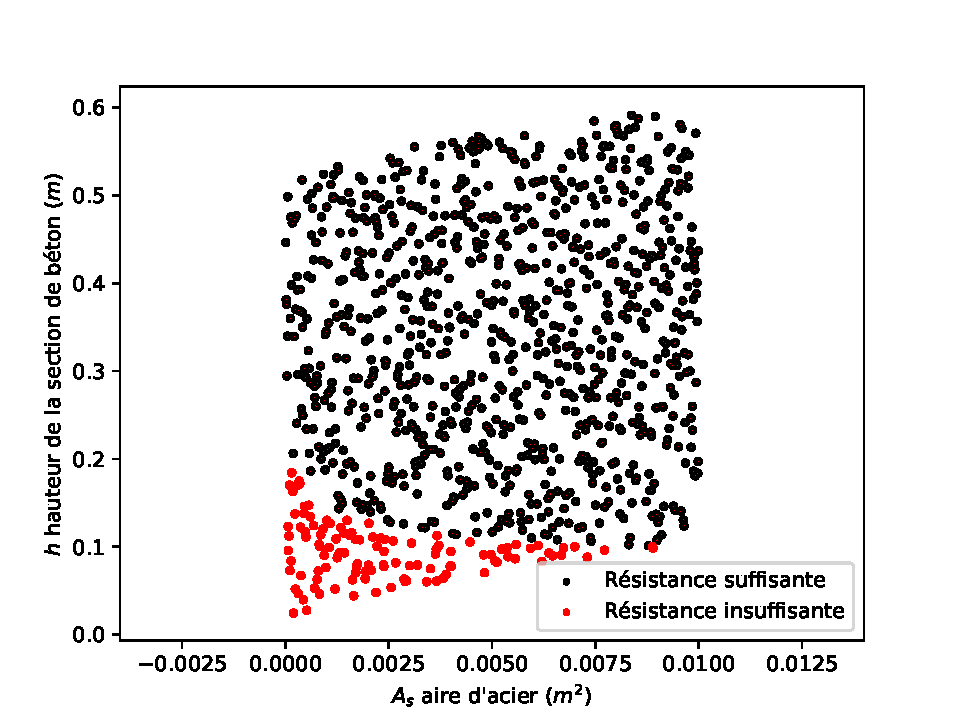
\includegraphics[width=.6\linewidth]{fig/faessel3}
  \caption{Results for the Faessel method (N=1000).}\label{fig:faessel3}
\end{figure}

\section{Instabilité au déversement}
\subsection{Eurocode 3}
Comme pour le flambement, l'Eurocode 3 donne une méthode permettant de vérifier la résistance au déversement d'un élément métallique.

\begin{dmath}
    M_{cr}=\frac{\pi^2 EI_z}{L^2}\sqrt{\frac{EI_w}{EI_z}+\frac{L^2GI_t}{\pi^2EI_z}}
\end{dmath}

\subsubsection{Résultats}
Voir Figure~\ref{fig:m1}.

\begin{figure}[!ht]
    \centering
    \includesvg[width=.8\linewidth]{fig/EC3MEdfy}
    \caption{Eurocode 3 en déversement, $x=M_{Ed}$, $y=f_y$.}\label{fig:m1}
\end{figure}

\listoffigures

\nocite{*}
\printbibliography
\end{document}
